\documentclass[10pt, a4paper,spanish]{article}

\usepackage[utf8]{inputenc}
\usepackage[spanish]{babel}

\usepackage[T1]{fontenc}

\usepackage[hmarginratio=1:1,top=32mm,columnsep=20pt]{geometry}
\usepackage[hang, small,labelfont=bf,up,textfont=it,up]{caption}

\usepackage{float}

\usepackage{amsmath}

\usepackage{enumitem}

\usepackage{graphicx}
\graphicspath{ {images/} }


\usepackage{titlesec}
\renewcommand\thesection{\Roman{section}}
\renewcommand\thesubsection{\Roman{subsection}}
\titleformat{\section}[block]{\large\scshape\centering}{\thesection.}{1em}{}
\titleformat{\subsection}[block]{\large}{\thesubsection.}{1em}{}

\usepackage{fancyhdr}
\pagestyle{fancy}
\fancyhead{}
\fancyfoot{}
\fancyhead[C]{ \today \ $\bullet$ Ingeniería del Conocimiento $\bullet$ Clips 3}
\fancyfoot[RO]{\thepage}

%-------------------------------------------------------------------------------
%	TITLE SECTION
%-------------------------------------------------------------------------------

\title{\vspace{-15mm}\fontsize{24pt}{10pt}\selectfont\textbf{Clips 3}} % Article title

\author{
	Fernández Angulo, Óscar \\
	\and
	García Prado, Sergio
}

\date{\today}

%-------------------------------------------------------------------------------

\begin{document}

	\maketitle % Insert title

	\thispagestyle{fancy} % All pages have headers and footers


%-------------------------------------------------------------------------------
%	TEXT
%-------------------------------------------------------------------------------

	\section{Sistema Cardiovascular Humano Basado en Probabilidad}

		\begin{enumerate}

			\item Así, cuando un paciente se queja de un dolor abdominal, una auscultación permite percibir un rumor abdominal y al palpar el abdomen del paciente se siente una masa pulsante, un aneurisma de la arteria abdominal probablemente (0.8) cause estos síntomas y evidencias clínicas.

			\item Si la presión sistólica del paciente supera los 140 mmHg, la presión del pulso es superior a 50 mmHg, y al auscultar al paciente se percibe un rumor sistólico o una dilatación del corazón, todo ello puede estar causado por una regurgitación aórtica (0.7).

			\item Como último ejemplo, si un paciente siente calambres en las piernas al andar, que desaparecen tras uno o dos minutos de descanso, la presencia de una estenosis en una de las arterias de las piernas es más que probable (0.9). A su vez, la estenosis suele deberse a un problema de arteriosclerosis (0.8), especialmente si el paciente pertenece a algún grupo de riesgo: obeso (0.8) o fumador durante más de 15 años (0.8) o edad superior a 50 años (0.6).

		\end{enumerate}

		\begin{figure}[H]
			\begin{center}
				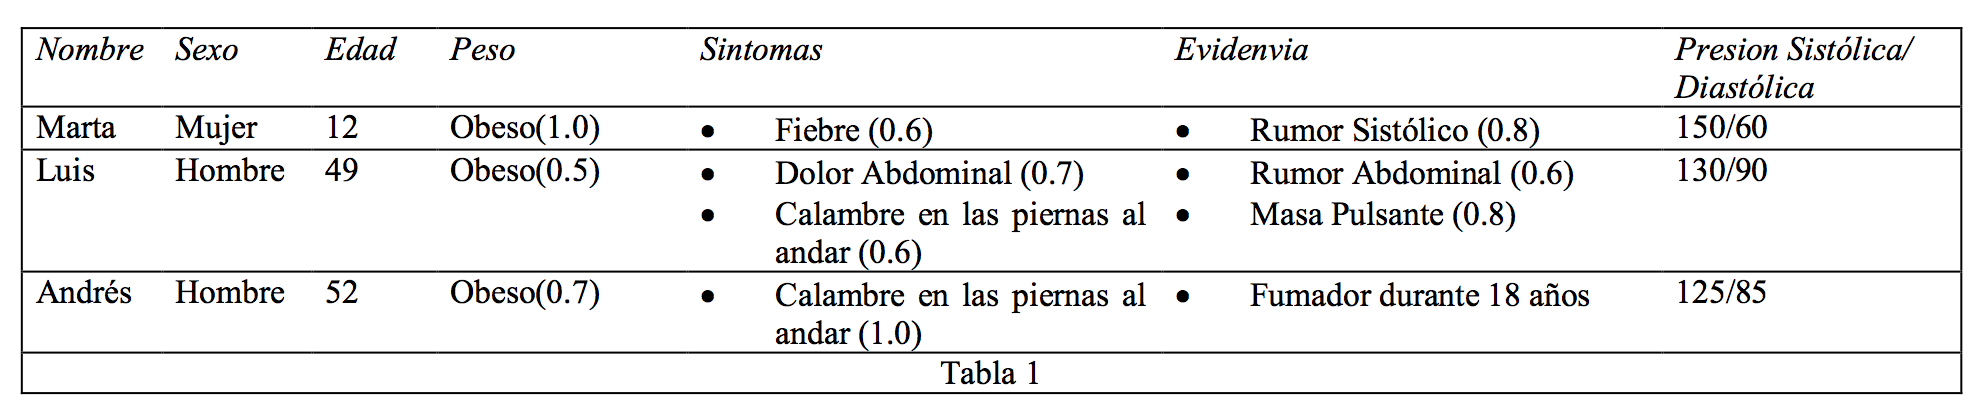
\includegraphics[width=0.9\textwidth]{table-1}
			\end{center}
		\end{figure}


\end{document}
